\documentclass{llncs}

\usepackage{url}
\usepackage{graphicx}
\usepackage{listings}
\usepackage{verbatim}
\usepackage[lined,linesnumbered,algochapter]{algorithm2e}
\usepackage{tikz}
\usetikzlibrary{arrows,automata}
\usepackage{xspace}
\usepackage{todonotes}          % Package for working draft comments
\usepackage{hyperref}           % Package for hyperlink references in the document


\usepackage[english]{babel}

\setcounter{secnumdepth}{2}
\setcounter{tocdepth}{3}

% define custom macros for specific formats or names
\newcommand{\uml}[1]{\texttt{#1}}
\newcommand{\cd}{\textsf{Class Diagram}}

\begin{document}
\pagestyle{plain}
\pagenumbering{roman}

\title{fUML Refactoring with EMF\footnote{This work has been created in the context of the course ``Advanced Model Engineering'' (188.952) in SS14.}}

\author{Sebastian Geiger (1127054) \and Kristof Meixner (9725208)}
\institute{Business Informatics Group\\Vienna Technical University}

\maketitle

\begin{abstract}
In this work we will present some ideas and concepts for the refactoring of fUML. The main contribution of this work is the extension of
existing UML refactorings to cover not only the static aspect of UML such as class diagrams but to also include refactorings for dynamic
parts such as activity diagrams. In this work we will present basic concepts for refactoring with EMF and show how model semantics can be
preserved through the use of OCL constraints. In the remainder of the paper we then present our tool chain and the used technologies
such as EMF and Ecore and how we used them for refactoring. We also present a discussion of EMF.Refactor, which shows how such refactorings
can be made available in the Eclipse GUIs such as the EMF tree editor or Papyrus.
\end{abstract}

\tableofcontents
\newpage

\pagenumbering{arabic}

\section{Introduction}
% INTRODUCTION Models are getting more important in model-based software development, model-driven software development,
% model-driven architecture Models thus need to have a good quality

Model-based software development or model-driven software development is not only an extensive field of research but
gets also more and more attention from the industry side. Nowadays models are not only used as visual explanations of
the underlying concepts but as source for the development process itself. Thus models need to provide an abstraction of
the represented domains in a high quality. Mohagheghi et al. \cite{DBLP:journals/infsof/MohagheghiDN09} discussed possible 
quality attributes of models in their work.

% UML is a modelling language for models provided by the OMG that supports various types of models

To represent formal models the OMG developed the UML \cite{man:UML} which by now advanced to an industry standard for modeling. With
these common semantics enriched models can be preserved over time and even reused.

% Models need to be changed in the development lifecycle

Nevertheless models might have to be revised over the lifecycle of the software. With todays trend to more agile software 
development such as eXtreme Programming \cite{DBLP:journals/computer/Beck99} or Scrum \cite{DBLP:journals/software/RisingJ00} 
changes on models have to be even more efficient which brings refactoring of models into account.

% Refactoring is behavior preserving changing that should also improve quality

Refactoring is a technique that originates from source code development but can also be applied to model engineering.
The goal is to introduce behavior preserving changes \cite{mast:REFOOF} that increase the quality and understandability
of the models.

% Refactoring must preserve the behavior of all model types

While refactoring source code respectively textual code applies to a single type of represenation in UML different
representations of models exist as various diagram types. This makes behavior preserving refactoring even harder as it
needs to span over those different types of diagrams and semantics.

% Behaviour preservation can be tested statically or dynamically UML can be analysed statically fUML is a modelling
% language for models provided by the OMG that also allows execution and thus can be analysed dynamically

To prove the correctness of models before and after refactoring different approachs exist. One is the static analysis of
UML models via metrics and the attempt to find model smells \cite{DBLP:conf/models/ArendtTW13} which can be done via
OCL \cite{man:OCL}. Another one is to verify that models can be executed and debugged in some way. The OMG introduced a subset 
of UML named fUML \cite{man:FUML} which narrowly defines semantics for class and acivity diagrams to make them executable. 
Mayerhofer \cite{DBLP:conf/icse/Mayerhofer12} in her work furthermore proposed a framework based on fUML that is able to execute
and debug those models.

% our approach is to combine both

The goal of this work is to introduce refactorings for fUML models, examine the requirements for co-refactoring of the
corresponding diagram types and define which co-changes have to be done to preserve the behavior. Our approach to prove
the correctness of the models after refactoring is twofold. On the one hand side we use pre- and postconditions
\cite{rob99} to define if the specific changes can be applied and that the models are semantically correct afterwards.
On the other hand side the models have to stay executable as well as traceable after the changes.

% we present a motivating example (class and activity diagrams) we provide some refactorings that target bothe diagram
% types we provide a how to test statically and dynamically, then refator and retest we provide a tool chain

% we provide some related work we provide a conclusion

The rest of the work is structured as follows. In section X we give an overview over fUML and provide a motivating
example of a model that is used throughout the paper. Section Y describes a selection of useful refactorings inspired by
Fowler \cite{fow99} and Markovic and Baar \cite{DBLP:journals/sosym/MarkovicB08} and their effects on class diagrams as
well as activity diagrams. In section Z we show which pre- and postcondition that are needed for the refactorings and
how we refactor the models. In section AA we describe the toolchain that we use to define the models, implement a set of
refactorings and test them. Related work is covered in section AC and a conclusion is drawn to summarize the paper.

% what is refactoring and what does it mean in the context of models?
% what is fuml? what does fuml consist for diagram types?
% what is ocl? why do we use it and what for?

%fUML adds semantics to UML models that make it possible to create semantically closed models which can be executed on the model level. With
%fUML classic refactorings are not enough to refactor those models as they do not support the refactoring of the dynamic aspects of models
%such as activity diagrams.

\section{Motivation}
% what do we want to achieve?
fUML is an extension of UML which builds on a subset of UML classes with the purpose of adding semantics to UML models such that they can
be executed on the model level. The dominant concept for this is the activity diagram. If a refactoring is performed on a UML model such
as a class diagram, then any activity diagram which is releated to the class diagram, has to be checked and possibly changed as well. In
section \ref{sec:fuml-refactoring} we will present some examples of fUML activity diagrams and present the implications that result from
changing class diagrams.

Since a refactoring changes the structure of a model it is important to ensure that all changes maintain the original semantics of the
model. Violating this requirement can result in models with either a different behavior, or in models which can no longer be executed.
To ensure semantic preservation, two main techniques can be used. First, the refactoring can be broken down into smaller steps, each of
which either guarantees to preseve the semantics of the model or makes it easier to verify that this is the case. Second, logical
constraints can be used to limit refactorings on models to only those cases where semantic preservation can be ensured. For this
purpose pre- and postconditions are specified with OCL constraints. A refactoring is then only applied if the original model satisfies
the precondition before the refactoring is applied and the postcondition after the refactoring has been completed. Such constrains must
be individually specified for each kind of refactoring that is to be performed, as such a part of this paper will discuss different OCL
constraints for the refactorings that we introduce.


In this paper we will present a set of refactorings and give examples of how each refactoring can be applied to a concrete model. 

% Why is it interesting to refactor models
% Why is it important in fUML that models remain consistent -> to preserve executability
% It is possible to use pre and post conditions in OCL to guarantee the semantic preservation of models during refactorings.

\section{Refactorings Examples}
% take model refactorings of markovic paper
% insurance example
% create example that supports all proposed refactorings

This section covers some general refactorings of UML class diagrams. As the basis of these refactorings an example from the insurance
domain is used. In the insurance business there are domain objects such as an insurance policy. Cars and trucks can be insured by 
adding them to the policy. There is an insurance company which has customers and employees and employees may purchase an insurance policy 
for one of their cars or trucks. Figure \ref{fig:classdiagramcomplex} shows a class diagram of such an insurance policy. This class 
diagram would benefit from several possible refactorings such as an \textit{extract superclass} which can be applied to both Car and Truck 
to extract a Vehicle class. A simple \textit{extract class} can be used on InsurancePolicy to extract the from and until dates into their
own InsurancePeriod class. As part of the \textit{extract superclass} refactoring two additional refactorings namely \textit{pull up 
attribute} and \textit{pull up method} are used to move the identical attributes and methods of both classes to the new superclass. As the 
attributes weight and registration are public, we can use \textit{encapsulate field} to make them private and provide getter and setter 
implementations. Finally the method addCar can be renamed into addVehicle with \textit{rename method} and the addTruck method can be 
removed with \textit{remove method}.

\begin{figure}[h!t]
 \centering
 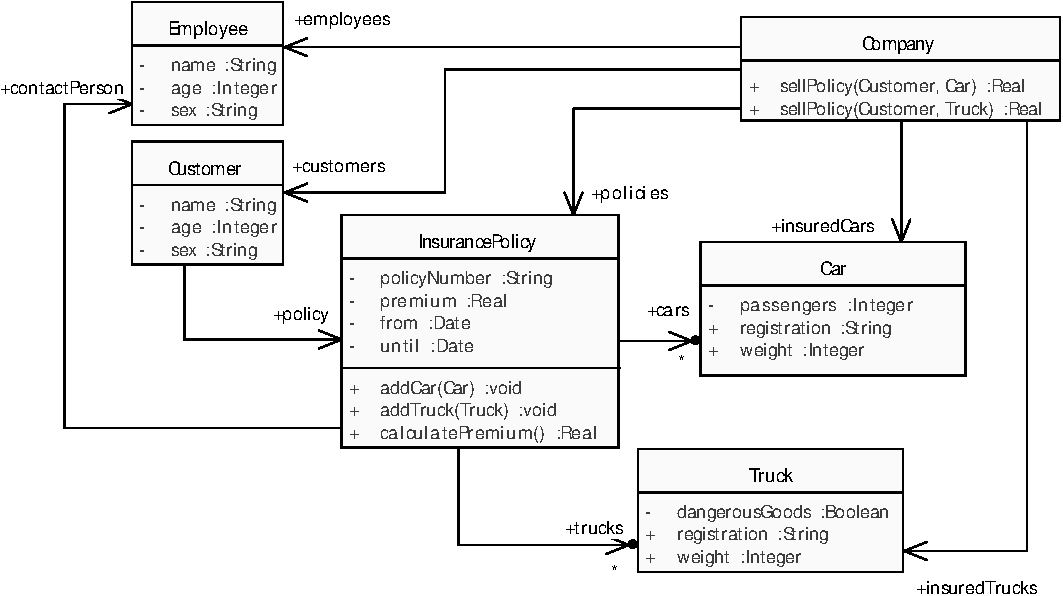
\includegraphics[scale=0.7]{images/ClassDiagramComplex.pdf}
 \caption{A car object that could benefit of extract class}
 \label{fig:classdiagramcomplex}
\end{figure}

For each of the methods the \textit{InsurancePolicy} and \textit{Company} classes a separate activity diagram exists which defines the
semantics of these methods. As some of them are quite similar we will present only the diagrams for addCar(), sellPolicy(Customer, Car) and calculatePremium().






Figure \ref{fig:complexcar} shows an example of a more complex car object which captures additinoal information about the owner which is allowed to drive the car. This example would benefit from an \textit{extract class} refactoring. The extract class refactoring would pull the members 
The policy allows to insure cars and trucks. Both Car and Truck have some attributes that are similar (weight, registration) and others that
are different (dangerousGoods, passengers). From the 

\begin{figure}[ht]
 \centering
 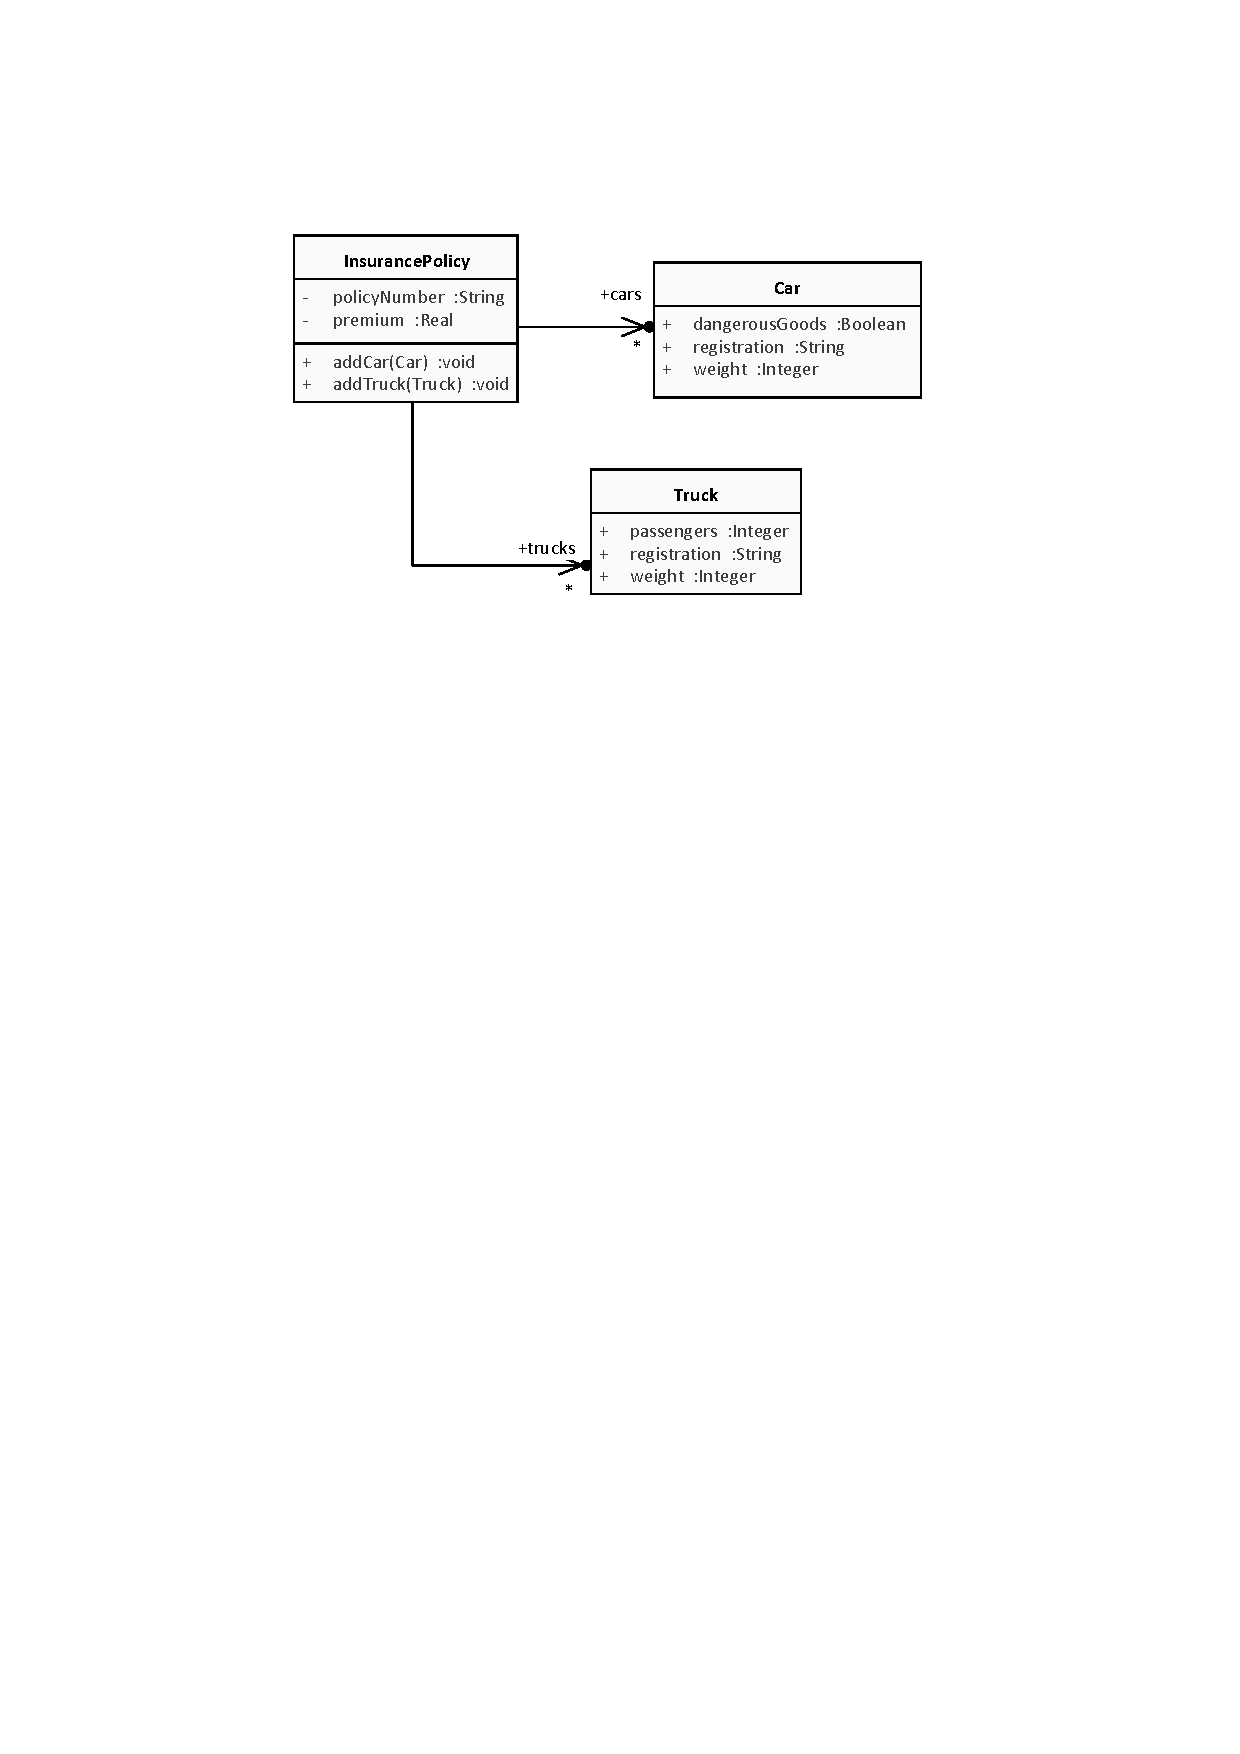
\includegraphics{images/addCar-class_diagram.pdf}
 \caption{Insurance policy class diagram}
 \label{fig:insurancepolicy}
\end{figure}

\begin{figure}
 \centering
 \begin{tabular}[]{l}
  \hline
  Extract class\\
  Extract superclass\\
  Rename Class\\
  Rename Method\\
  Rename Variable\\
  Add / Remove Parameter\\
  Encapsulate Field\\
  Pull up attribute\\
  Pull up operation\\
  Pull up association end\\
  Remove unused class\\
  \hline
 \end{tabular}
 \caption{Refactoring examples}
 \label{fig:refactoringlist}
\end{figure}

In this section we will present some general refactorings such as the ``extract superclass'' refactoring. A list of example refactorings
is presented in figure \ref{fig:refactoringlist}.




\begin{figure}[ht]
 \centering
 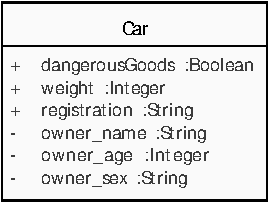
\includegraphics{images/ComplexCar-class_diagram.pdf}
 \caption{A car object that could benefit of extract class}
 \label{fig:complexcar}
\end{figure}


\section{Refactoring of fUML diagrams}
\label{sec:fuml-refactoring}
% abstract syntax of fUML and changes in diagrams
% ecore and ocl (with code examples)
In this section we will present some general refactorings

\begin{figure}[ht]
 \centering
 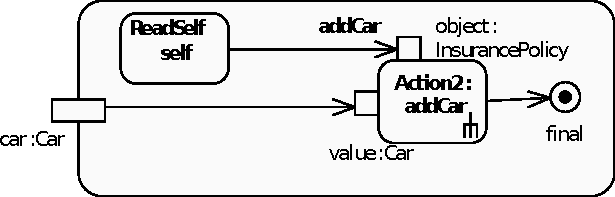
\includegraphics{images/addCar-activity_diagram}
\end{figure}

\section{Tool chain and implementation}
For our tool chain we have relied on the moliz\footnote{source...} repository, mainly for the ability to execute the fUML models with
a virtual machine. The models are stored as XMI 
% usage of fUML reference implementation of BIG
% how to load models?
% how to execute models?
% how to apply queries and changes?

\subsection{Model refactoring}
Describe our tool chain, how we created models, how we load them, what information of the abstract syntax we use for refactoring, etc.

\subsection{GUI Integration}
Describe what we did with EMF.Refactor.

\section{Related Works}
% Refactoring of prgram code

In this section we give an overview on the related work. Refactoring in a general way with preconditions was described
by Opdyke \cite{mast:REFOOF} in his master thesis and stated more precisely by Roberts \cite{rob99} who also introduced
postconditions for refactorings. Fowler \cite{fow99} generated an extensive yet simple to understand catalog of
refactorings for Java and Ruby which can be be adapted to model refactorings.

% Refactoring of models and OCL Code analysis via OCL

Suny{\'e} et. al. \cite{DBLP:conf/uml/SunyePTJ01} described how several refactorings can be applied to \textit{UML}
diagrams and introduced OCL as a possiblity to specify pre- and postconditions. Gorp et al. \cite{gorp03} extends the
discussion with the usage of \textit{OCL} for additinal analysis such as code smells of models.

% Code execution via fUML

Despite of the further discussion of model refactoring (\cite{DBLP:conf/uml/CorreaW04}, \cite{DBLP:conf/ershov/BaarM06},
\cite{DBLP:journals/ase/ArendtT13}) most authors concetrate on static analysis and class diagram representations of
models. Dynamic analysis of models by execution and debugging \textit{fUML} models is discussed by Mayerhofer
\cite{DBLP:conf/icse/Mayerhofer12} and provides the basis for the approach discussed here. Mayerhofer et al.
\cite{DBLP:conf/models/MayerhoferLK12} furthermore introduce a runtime model and an
implementation\footnote{http://www.modelexecution.org} that is capable to test the models and directly show impacts of
refactorings.

% Refactoring implementation with EMF Refactor

Arendt and Taentzer \cite{DBLP:journals/ase/ArendtT13} present a framework that is based on \textit{Eclipse} and the
\textit{Eclipse Modelling Framework} which allows static model analysis and refactorings that are implemented in
different languages (Java, OCL \& Henshin) and can be directly extended in \textit{Eclipse}.


\section{Conclusion}
We conclude this paper with...

\bibliographystyle{acm}
\bibliography{references}

\end{document}
